\chapter{Probability Theory}

Homomorphic encryption schemes are based on noise. As we will see in Subsection \ref{subsec:LWE}, noise can be sampled from discrete spaces in accordance with a distribution. Since distributions are central in cryptography, it is important they are understood. A distribution is a probability measure on a measurable space $(S, \mathcal{S})$. Typically, probability distributions are associated with random variables; however, in the absence of random variables, distributions are understood as a specified measure function on the given measurable space (See \cite[pp. 83]{kallenberg-probability}).
\begin{definition}[Discrete distribution measure of a random variable]
Consider a probability space $(\Omega, \mathcal{F}, \operatorname{Pr})$ and a discrete measurable space $(S,\mathcal{S})$. Let $X \colon \Omega \mapsto S$ be a random variable. The discrete distribution measure of $X$, or simply \emph{distribution} of $X$, $\chi$ is defined as follows
\begin{equation*}
\begin{aligned}
    \chi \colon \mathcal{S} &\to [0,1]\\
    \{x\} &\mapsto \operatorname{Pr}[X = x]
\end{aligned}
\end{equation*}
We say that $\chi$ is the distribution or \emph{law} of $X$, denoted $\mathcal{L}(X)$. 
\end{definition}
\begin{remark}
    Since $\chi$ is a measure on a discrete space, the description of the singletons are sufficient. More explicitly, $\chi(A) = \sum_{x \in A} \operatorname{Pr}[X = x]$ for $A \in \mathcal{S}$
\end{remark}
A distribution measure for a random variable is a probability measure on the sample space $(S,\mathcal{S})$, as opposed to on the outcome space $(\Omega, \mathcal{F})$. For a given probability space, any random variable $X$ defined on it has a distribution associated with it. We write $x \leftarrow X$ or $x \leftarrow \chi$ for sampling the outcome $x$ from $X$ assuming $\chi$ is its distribution. When $X$ is a space we mean that $x$ is uniformly sampled from $X$.

\begin{definition}[Ensembles] \label{def:prob-ensemble}
    Let $I$ be a countable index set. A \emph{probability ensemble} indexed by $I$ (or just ensemble) is a sequence of random variables $(X_i)_{i \in I}$. A \emph{distribution ensemble} indexed by $I$ is a sequence of distributions $(\chi_i)_{i \in I}$
\end{definition}
In this paper we will exclusively use $\mathbb{N}$ as the index set.
For example, the encryption function is a random variable (PPT algorithm), meaning that a single message $m$ corresponds to many valid ciphertexts. By varying the security parameter of the scheme we construct the probability ensemble $\{Enc(pk,m)\}_{pk \in \mathbb{N}}$
\begin{definition}[Statistical distance] \label{def:statistical-distance}
    Let $S_n$ be finite set for all $n \in \mathbb{N}$ and let $X = (X_n \colon \Omega_n \to S_n)_{n \in \mathbb{N}}$, $Y = (Y_n \colon \Omega_n \to S_n)_{n \in \mathbb{N}}$ be two ensembles. The \emph{statistical distance} is defined as
    \begin{equation*}
        \Delta_{X,Y}(n) \stackrel{\mathrm{def}}{=} \frac{1}{2} \sum_{\alpha \in S_n} |\operatorname{Pr}[X_n = \alpha] - \operatorname{Pr}[Y_n = \alpha]|.
    \end{equation*}
    Let $\chi = \{\chi_n\}_{n \in \mathbb{N}}$, $\psi = \{\psi_n\}_{n \in \mathbb{N}}$ be two discrete distribution ensembles on the same measurable spaces $\{(S_n, \mathcal{S}_n)\}_{n \in \mathbb{N}}$. The statistical distance is defined as
    \begin{equation*}
    \begin{aligned}
        \Delta_{\chi, \psi}(n) \stackrel{\mathrm{def}}{=} \frac{1}{2} \sum_{\alpha \in S_n} |\chi_n(\{\alpha\}) - \psi_n(\{\alpha\})|
    \end{aligned}
    \end{equation*}
\end{definition}
\begin{remark}
    This definition for distribution ensembles assumes every singleton is measurable. A more general definition is $\Delta(\chi, \psi) \stackrel{\mathrm{def}}{=} \sup _{A \in \mathcal{S}}|\chi(A)-\psi(A)|$ 
\end{remark}

\begin{definition}[Negligible function]
    Let $f \colon \mathbb{N} \to [0,1]$. $f$ is negligible if for all positive polynomials $p(\cdot)$, there exists an $N$ such that for all $n>N$, $f(n) < \frac{1}{p(n)}$. We say $f = \operatorname{negl}(n)$.
\end{definition}
\begin{definition}[Perfectly indistinguishable] \label{def:perfectly-indistinguishable}
    Two ensembles (probability or distribution) $X$ and $Y$ are \emph{perfectly indistinguishable} if $\Delta_{X,Y}(n) = 0$ for all $n$.
\end{definition}
\begin{definition}[Statistically indistinguishable] \label{def:statistically-indistinguishable}
    Two ensembles (probability or distribution) $X$ and $Y$ are \emph{statistically indistinguishable} if $\Delta_{X,Y}(n) = \operatorname{negl}(n)$.
\end{definition}
 A desirable property of encryption schemes is to make it unfeasible for adversaries to distinguish encryptions. For two random variables (or distributions) $X$ and $Y$, we want every adversary $C$ to not be able to distinguish samples from $X$ and $Y$. More precisely, an adversary tasked with identifying whether given samples are from $X$ ($C$ outputs 0) or from $Y$ ($C$ outputs 1) should have roughly the same probability of success irrespective of which the samples are generated from. The formal definition is as follows:
\begin{definition}[Computationally indistinguishable \cite{Gol01}] \label{def:computationally-indistinguishable}
    Two ensembles (or distribution ensembles) $X$ and $Y$ are computationally indistinguishable if, for every polynomial-size circuit family $C = \{C_n\}_{n \in \mathbb{N}}$, $$\operatorname{Adv}_{X,Y}(n) \stackrel{\mathrm{def}}{=} |\operatorname{Pr}[C(X_n) = 1] - \operatorname{Pr}[C(Y_n) = 1]| = \operatorname{negl}(n).$$
\end{definition}
$C(X_n), C(Y_n)$ means that the adversary has access to random oracle returning a sample from $X_n$ and $Y_n$ respectively. The point is that, for every adversary $C$ guessing the samples are from one of the random variables or distributions (1 in this case represents from $Y_n$), the probability of being correct is, up to negligible error, equal to the probability of being incorrect. For example, an adversary always guessing 1 has 100\% probability of being incorrect when given samples from $X_n$ and 100\% probability of being correct when given samples from $Y_n$. The intuition is that the sample does not make a noticable difference on the guess and that the advantage in distinguishing samples goes to zero fast (faster than the inverse of all polynomials).

Perfect distinguishability implies statistical indistinguishability as 0 is negligible. Statistical indistinguishability implies computational indistinguishability. To see why, assume $\Delta_{X,Y}(n) = \operatorname{negl}(n)$ and consider any circuit family $C$. Since $X_n$ and $Y_n$ are defined on the same space we have
\begin{equation*}
\begin{aligned}
    \operatorname{Adv}_{X,Y}(n) &= |\operatorname{Pr}[C(X_n) = 1] - \operatorname{Pr}[C(Y_n) = 1]|\\
        &\leq \sum_{\alpha \in S_n} | \operatorname{Pr}[C(X_n = \alpha) = 1 \; | \; X_n = \alpha]\operatorname{Pr}[X_n = \alpha] \\
        &\phantom{=} \qquad - \operatorname{Pr}[C(Y_n = \alpha) = 1 \; | \; Y_n = \alpha]\operatorname{Pr}[Y_n = \alpha] | \\
        &\leq \sum_{\alpha \in S_n} | \operatorname{Pr}[X_n = \alpha] - \operatorname{Pr}[Y_n = \alpha]| = 2\Delta_{X,Y}(n) = \operatorname{negl}(n)
\end{aligned}
\end{equation*}
where the first inequality is due to the triangle inequality and the second is due to conditional probability being upper bounded by 1. Intuitively, there does not exist enough distinguishable outcomes to distinguish the ensembles even if there exists an adversary that always correctly recognize an outcome from $X$ and $Y$ respectively.
\subsection*{Distributions for noise in HE}
To add discrete noise to ciphertexts, it is typical to use the discretized Gaussian distribution introduced by Micciancio and Regev \cite{disc-gauss}. Since this distribution is used so frequently, we give a brief presentation of it here. A continuous Gaussian distribution in $\mathbb{R}^n$ centered at $\vec{c}$ where each coordinate is independently sampled from normal distirbution with standard deviation $\sigma$, then the multivariate Gaussian distribution is simplified to $\rho_{\vec{c}}(\vec{x}; \sigma)=\frac{1}{\left(2 \pi \sigma^2\right)^{n / 2}} \exp \left(-\frac{1}{2 \sigma^2} \| \vec{x}-\vec{c} \| ^2\right)$. By introducing the scale factor $s \stackrel{\mathrm{def}}{=} \sqrt{2\pi}\sigma$ we get $\rho_{s, \vec{c}}(\vec{x})=\frac{1}{s^n} \exp \left(-\frac{\pi}{s^2} \| \vec{x}-\vec{c} \| ^2\right)$.
The goal is to discretize the gaussian over lattices, see Section \ref{sec:lattices}, by restricting the domain to lattice points. For a given lattice $L \subset \mathbb{R}^n$ we define the normalization constant $\rho_{s, \vec{c}}(L) \stackrel{\mathrm{def}}{=} \sum_{\vec{x} \in L} \rho_{s, \vec{c}}(\vec{x})$.
\begin{definition}[Discrete Gaussian distribution]\label{Disc-Gauss}
    Let $L \subset \mathbb{R}^n$ be a lattice. Then the discrete gaussian distribution is defined as
    \begin{equation*}
        \forall \vec{x} \in L \colon \quad \textrm{D}_{L, s, \vec{c}}(\vec{x}) \stackrel{\mathrm{def}}{=} \frac{\rho_{s, \vec{c}}(\vec{x})}{\rho_{s, \vec{c}}(L)}.
    \end{equation*}            
\end{definition}
\begin{definition}[$\beta$-bounded distribution]
    Let $\chi = \{\chi_n\}_{n\in \mathbb{N}}$ be a distribution ensemble over the integers. $\chi$ is $\beta$-bounded if $x \leftarrow \chi_n \implies |x| < \beta$
\end{definition}
\begin{remark}
    It is also possible (and common) to define a $\beta$-bounded distribution such that $x \geq \beta$ with negligible probability.
\end{remark}
\begin{figure}
    \centering
    \hypertarget{fig:discrete-gauss}{}
    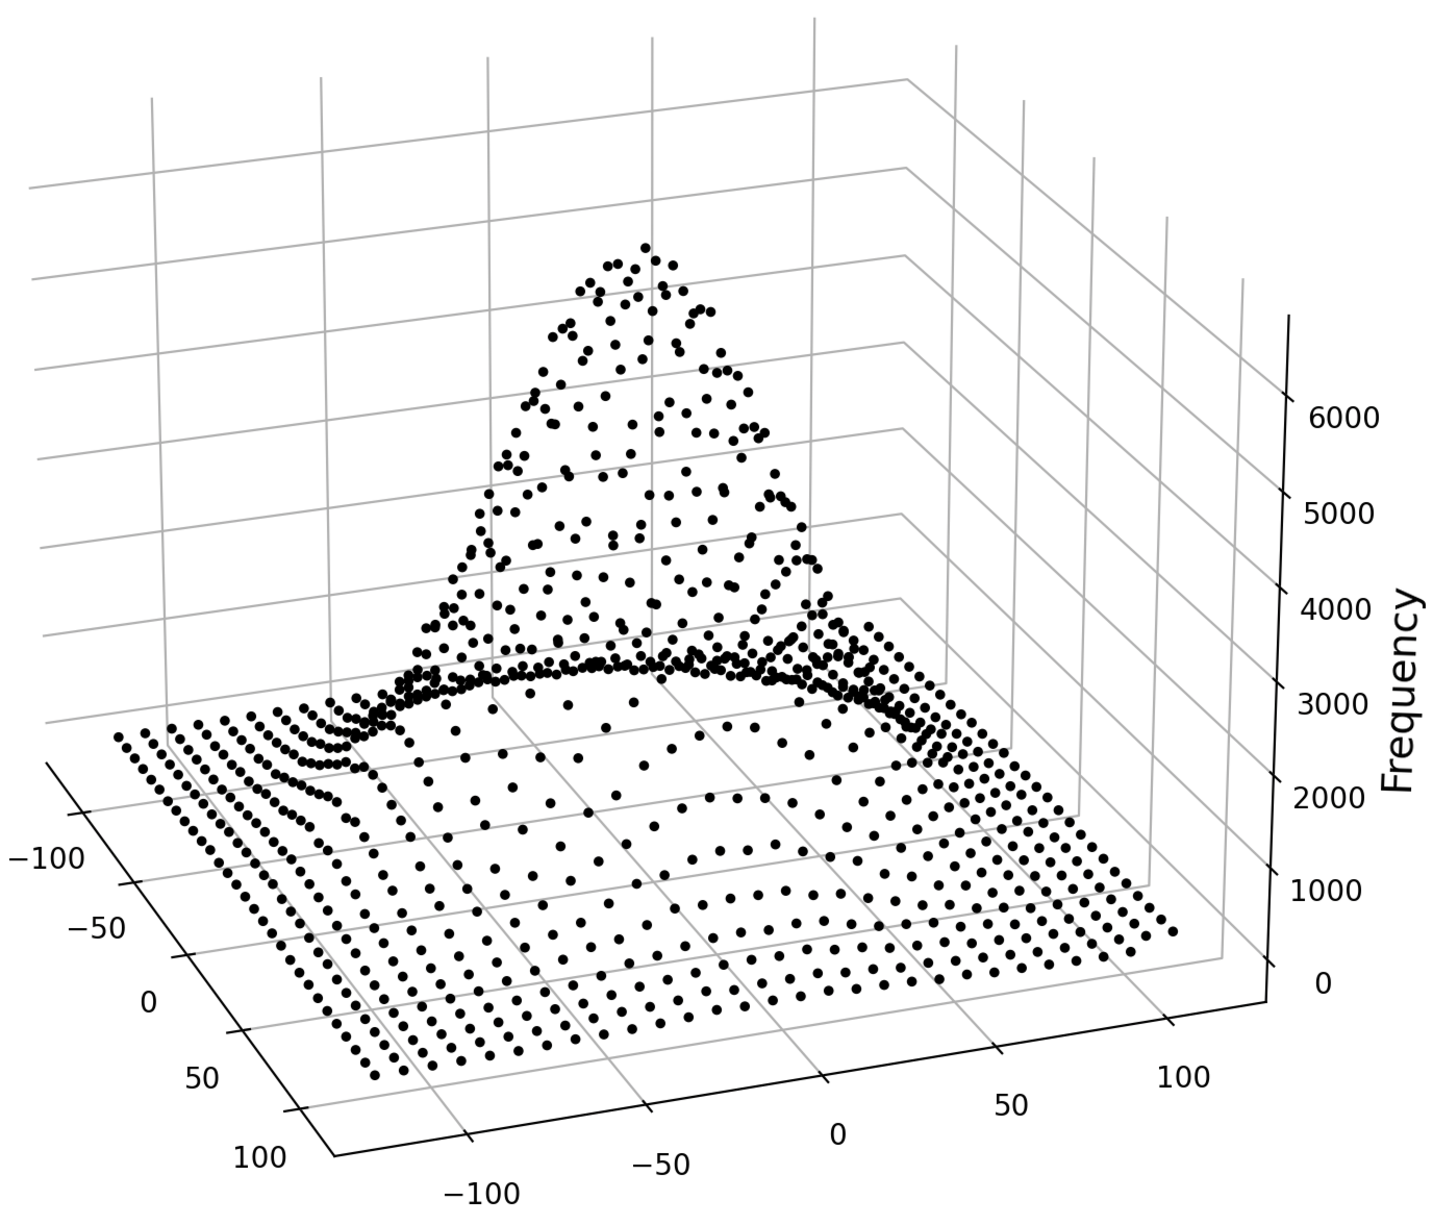
\includegraphics[width=0.65\textwidth]{figures/D-G-2d-a_is_100-n_1000000.pdf}
    \caption*{\textbf{Figure 1}: Discrete Gaussian distribution $\textrm{D}_{\mathbb{Z}^2, 100, \vec{0}}$ with 1 million samples. Every point has integer coordinates. See code in Appendix \ref{app:code}.}
\end{figure}
